\documentclass{../cssheet}

%--------------------------------------------------------------------------------------------------------------
% Basic meta data
%--------------------------------------------------------------------------------------------------------------

\title{Taxigeometrie}
\author{Prof. Dr. Christian Spannagel}
\date{\today}
\hypersetup{%
    pdfauthor={\theauthor},%
    pdftitle={\thetitle},%
    pdfsubject={Aufgabenblatt Geometrie},%
    pdfkeywords={geometrie}
}


%--------------------------------------------------------------------------------------------------------------
% document
%--------------------------------------------------------------------------------------------------------------

\begin{document}
\printtitle

\begin{center}
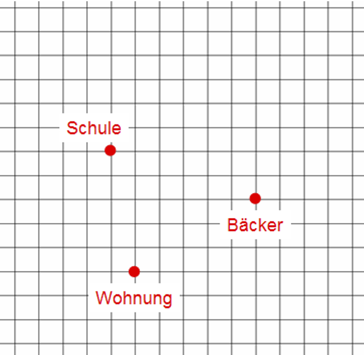
\includegraphics[width=7cm]{stadtplan.png}
\end{center}

\textbf{Aufgabe 1:}  Zeichne drei verschiedene Wege von der Wohnung zum Bäcker ein.

\textbf{Aufgabe 2:}  Wie lang ist der kürzeste Weg von der Wohnung zum Bäcker (\glqq{}Taxiabstand\grqq{})? Gibt es mehrere solche Wege?

\textbf{Aufgabe 3:}  Wie viele kürzeste Wege gibt es von der Wohnung zur Schule? Wie viele kürzeste Wege gibt es von der Wohnung zum Bäcker? 

\textbf{Aufgabe 4:} Zeichne alle Punkte ein, die von der Schule den Taxiabstand $3$ haben. Wie könnte man diese Punktmenge nennen?

\textbf{Aufgabe 5:} Zeichne alle Punkte ein, die von der Schule und der Wohnung gleich weit entfernt sind. Zeichne alle Punkte ein, die von der Schule und dem Bäcker gleich weit entfernt sind. Wie könnte man diese Punktmengen jeweils nennen? Sehen diese Punktmengen immer \glqq{}so\grqq{} aus? Suche nach Sonderfällen!

\textbf{Aufgabe 6:} Angenommen, es handelt sich bei dem Stadtplan um ein Koordinatengitter mit dem Ursprung im Taxipunkt ganz links unten. Wie kann man den Taxiabstand $d_T(A,B)$ zweier Punkte $A$ und $B$ berechnen? Wie berechnet man den Abstand zweier Punkte $d_E(A,B)$ in der euklidischen Geometrie? Welche anderen Abstandsmaße in anderen Geometrien wären denkbar?

\textbf{Aufgabe 7:} Wenn $d_T(A,B) = d_T(C,D)$, gilt dann auch $d_E(A,B)=d_E(C,D)$? Und umgekehrt? Unter welchen Bedingungen gilt: $d_T(A,B) = d_E(A,B)$? Ist es immer wahr, dass $d_E(A,B) \leq d_T(A,B)?$

\textbf{Aufgabe 8:} Was wäre ein vernünftiger Wert für die Zahl $\pi$ in der Taxigeometrie? 

Die Aufgaben orientieren sich an Aufgaben aus: Krause, E. F. (1986). \emph{Taxicab Geometry}. New York: Dover Publications.


\newpage

\printlicense

\printsocials


\end{document}
